\section{Debugger/GUI}
\label{sec:debugger}

\vonda comes with a GUI \citep{rudibuggerThesis} that helps navigating, compiling and editing the source files belonging to a project. It can also be attached to your \vonda project at runtime to support debugging by logging the evaluation of rule conditions.

\begin{figure}[thb]

  \centering
  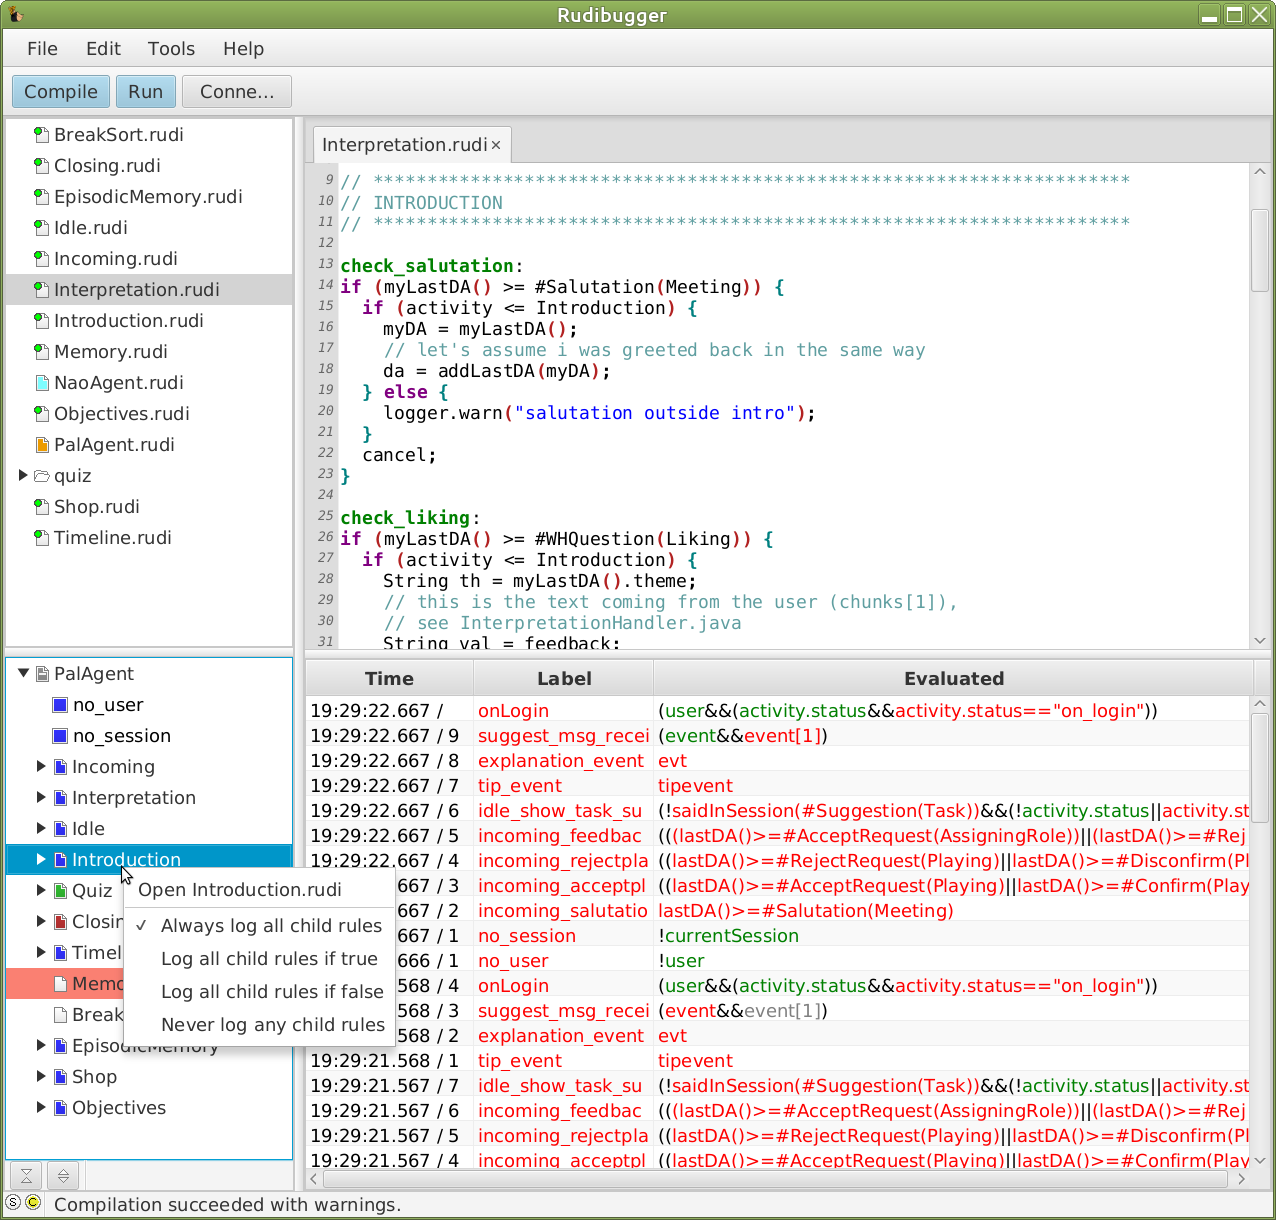
\includegraphics[width=.8\textwidth]{VondaGui.png}
  \caption{The \vonda GUI window}
  \label{vondagui}
\end{figure}

For further details, please take a look into rudibuggers own documentation. The project can be found on \url{https://github.com/yoshegg/rudibugger}.